
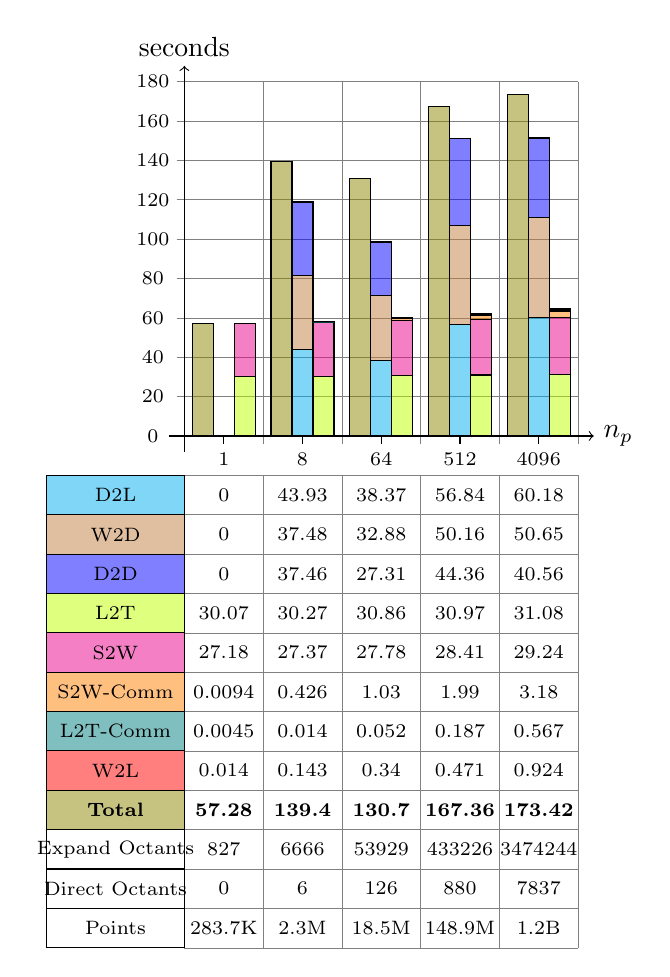
\begin{tikzpicture}[scale=1.0]

\draw[very thin, color=gray, xstep=1, ystep=0.5] (-0.1,-0.1) grid (5, 4.5);
\draw[->] (-0.2, 0) -- (5.2, 0) node[right] {$n_p$};
\draw[->] (0, -0.2) -- (0, 4.7) node[above] {seconds};

\newdimen\yscale

\yscale= 0.025 cm

\foreach \pos/\label in {0.5/1, 1.5/8, 2.5/64, 3.5/512, 4.5/4096} {
\draw (\pos,0) -- (\pos,-0.1) (\pos cm,-2.5ex) node [anchor=base,fill=white,inner sep=1pt]  {\scriptsize{\label}};
}

\foreach \label in {0, 20, ..., 180} {
 \draw (-0.4, \label\yscale) node {\scriptsize{\label}};
}

\draw[very thin, color=gray, xstep=1, ystep=0.5] (0, -6.5) grid (5, -0.5);

\draw[fill=cyan, fill opacity=0.5] (-1.75, -1.0) rectangle +(1.75, 0.5);
\draw (-0.875, -0.75) node {\scriptsize{D2L}};

\draw[fill=brown, fill opacity=0.5] (-1.75, -1.5) rectangle +(1.75, 0.5);
\draw (-0.875, -1.25) node {\scriptsize{W2D}};

\draw[fill=blue, fill opacity=0.5] (-1.75, -2.0) rectangle +(1.75, 0.5);
\draw (-0.875, -1.75) node {\scriptsize{D2D}};

\draw[fill=lime, fill opacity=0.5] (-1.75, -2.5) rectangle +(1.75, 0.5);
\draw (-0.875, -2.25) node {\scriptsize{L2T}};

\draw[fill=magenta, fill opacity=0.5] (-1.75, -3.0) rectangle +(1.75, 0.5);
\draw (-0.875, -2.75) node {\scriptsize{S2W}};

\draw[fill=orange, fill opacity=0.5] (-1.75, -3.5) rectangle +(1.75, 0.5);
\draw (-0.875, -3.25) node {\scriptsize{S2W-Comm}};

\draw[fill=teal, fill opacity=0.5] (-1.75, -4.0) rectangle +(1.75, 0.5);
\draw (-0.875, -3.75) node {\scriptsize{L2T-Comm}};

\draw[fill=red, fill opacity=0.5] (-1.75, -4.5) rectangle +(1.75, 0.5);
\draw (-0.875, -4.25) node {\scriptsize{W2L}};

\draw[fill=olive, fill opacity=0.5] (-1.75, -5.0) rectangle +(1.75, 0.5);
\draw (-0.875, -4.75) node {\scriptsize{\textbf{Total}}};

\draw (-1.75, -5.5) rectangle +(1.75, 0.5);
\draw (-0.875, -5.25) node {\scriptsize{Expand Octants}};

\draw (-1.75, -6.0) rectangle +(1.75, 0.5);
\draw (-0.875, -5.75) node {\scriptsize{Direct Octants}};

\draw (-1.75, -6.5) rectangle +(1.75, 0.5);
\draw (-0.875, -6.25) node {\scriptsize{Points}};

\newdimen\mypos
\newdimen\myoff

\foreach \pos/\vala/\valb/\valc/\vald/\vale/\valf/\valg/\valh/\vali/\valj/\valk/\vall in {
 0/0/0/0/30.07/27.18/0.0094/0.0045/0.014/57.28/827/0/283.7K,
 1/43.93/37.48/37.46/30.27/27.37/0.426/0.014/0.143/139.4/6666/6/2.3M,
 2/38.37/32.88/27.31/30.86/27.78/1.03/0.052/0.34/130.7/53929/126/18.5M,
 3/56.84/50.16/44.36/30.97/28.41/1.99/0.187/0.471/167.36/433226/880/148.9M,
 4/60.18/50.65/40.56/31.08/29.24/3.18/0.567/0.924/173.42/3474244/7837/1.2B
  } { 

\mypos=\pos cm
\advance \mypos by 0.5 cm

\draw (\mypos, -0.75 cm) node {\scriptsize{\vala}};
\draw (\mypos, -1.25 cm) node {\scriptsize{\valb}};
\draw (\mypos, -1.75 cm) node {\scriptsize{\valc}};
\draw (\mypos, -2.25 cm) node {\scriptsize{\vald}};
\draw (\mypos, -2.75 cm) node {\scriptsize{\vale}};
\draw (\mypos, -3.25 cm) node {\scriptsize{\valf}};
\draw (\mypos, -3.75 cm) node {\scriptsize{\valg}};
\draw (\mypos, -4.25 cm) node {\scriptsize{\valh}};
\draw (\mypos, -4.75 cm) node {\scriptsize{\textbf{\vali}}};
\draw (\mypos, -5.25 cm) node {\scriptsize{\valj}};
\draw (\mypos, -5.75 cm) node {\scriptsize{\valk}};
\draw (\mypos, -6.25 cm) node {\scriptsize{\vall}};

\advance \mypos by -0.4 cm
\myoff=0 cm

%Total

\draw[fill=olive, fill opacity=0.5] (\mypos, \myoff) rectangle +(0.266667, \vali\yscale);

%Direct

\advance \mypos by 0.266667 cm

\myoff=0 cm

\draw[fill=cyan, fill opacity=0.5] (\mypos, \myoff) rectangle +(0.266667, \vala\yscale);
\advance \myoff by \vala\yscale

\draw[fill=brown, fill opacity=0.5] (\mypos, \myoff) rectangle +(0.266667, \valb\yscale);
\advance \myoff by \valb\yscale

\draw[fill=blue, fill opacity=0.5] (\mypos, \myoff) rectangle +(0.266667, \valc\yscale);

%Expand

\advance \mypos by 0.266667 cm

\myoff=0 cm

\draw[fill=lime, fill opacity=0.5] (\mypos, \myoff) rectangle +(0.266667, \vald\yscale);
\advance \myoff by \vald\yscale

\draw[fill=magenta, fill opacity=0.5] (\mypos, \myoff) rectangle +(0.266667, \vale\yscale);
\advance \myoff by \vale\yscale

\draw[fill=orange, fill opacity=0.5] (\mypos, \myoff) rectangle +(0.266667, \valf\yscale);
\advance \myoff by \valf\yscale

\draw[fill=teal, fill opacity=0.5] (\mypos, \myoff) rectangle +(0.266667, \valg\yscale);
\advance \myoff by \valg\yscale

\draw[fill=red, fill opacity=0.5] (\mypos, \myoff) rectangle +(0.266667, \valh\yscale);

}

\end{tikzpicture}

